\chapter{Entregable 4}

\subsection{Ejercicio 1}

Escoja una de las bases de datos de clasificación para el trabajo de las dispuestas en Moodle. Se entiende que además de pasarla a formato .arff ya ha aplicado el preprocesamiento necesario en función del fichero "Pistas sobre los datasets con posible preprocesamiento a simple vista.pdf", en el caso que sea una de las bases de datos que lo requiera.

Cargue la base de datos y ejecute el algoritmo C4.5 usando un 75\% para entrenar y un 25\% para generalizar, con los parámetros por defecto.
Analice y muestre el árbol obtenido con los parámetros por defecto: nodo principal, número de nodos u hojas, variables presentes y omitidas. Comente también los resultados de las métricas obtenidas.

Para comenzar con el ejercicio hemos escogido la base de datos proporcionada por Moodle que anteriormente hemos pasado a formato .arff, esta base de datos consta de doce atributos de tipo numérico por lo cual deberíamos de aplicarle una discretización para así pasarlos a nominal, sin embargo esta es una de las ventajas del algoritmo empleado que a diferencia del algoritmo ID3 este, el C4.5 discretiza automáticamente por lo que para aplicarlo solo hemos tenido que modificar el tanto por ciento que deseamos destinar a entrenamiento tal y como muestra la figura de abajo.

\begin{figure}[H]
    \centering
    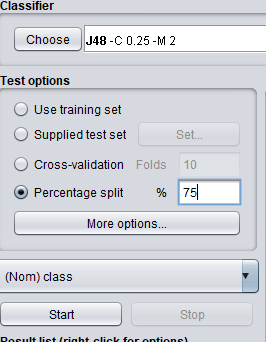
\includegraphics[width=\textwidth]{img/Porcentaje.PNG}
    \caption{Aplicación del 75\% de entrenamiento}
    
\end{figure}

A continuación mostraremos el árbol obtenido para comentar sus resultados así como sus reglas pertinentes y algunos datos de su estructura.

\begin{figure}[H]
    \centering
    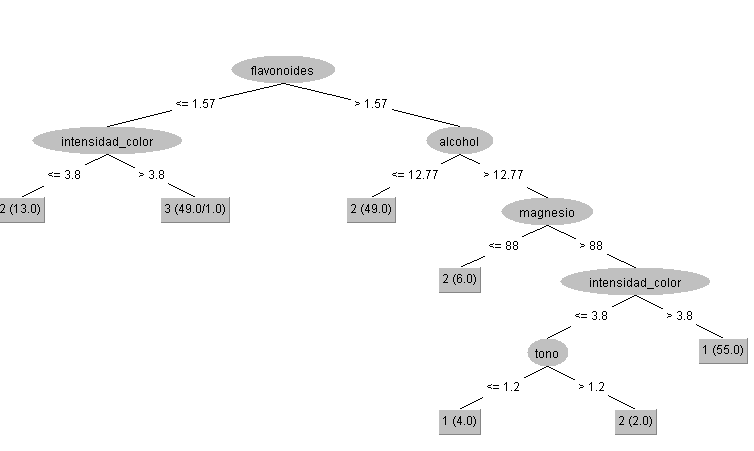
\includegraphics[width=\textwidth]{img/Tree.PNG}
    \caption{Árbol obtenido por el algoritmo C4.5}
    
\end{figure}

\begin{figure}[H]
    \centering
    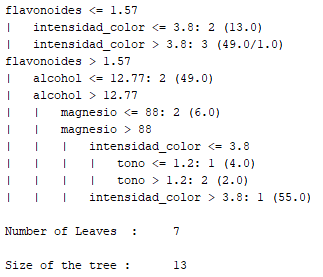
\includegraphics[width=\textwidth]{img/Reglas.PNG}
    \caption{Reglas propias del árbol}
    
\end{figure}

Cómo vemos en las figuras de arriba nuestro árbol está formado por seis nodos que corresponde con seis análisis de variable que son, flavonoides, intensidad\_color, alcohol, magnesio, y tono. Comenzamos analizando flavonoide ya que es esta la que nos produce una menor entropía. Además poseemos siete nodos terminales u hoja los cuales determinan a que clase pertenece la instancia analizada según el camino o reglas seguidas. También podemos destacar que hay alguna variables las cuales no aparecen lo que nos quiere decir que no son influyentes a la hora de clasificar una instancia, estas son, ácido\_malico, ceninaz, alcalinidad\_cenizas, fenoles\_totales, fenoles\_no\_flavonoides, proantocianinas y OD280.

Con respecto a las métricas debemos destacar un alto valor de CCR con un 93.1818\% además de un valor del estadístico Kappa de 0.8966 muy superior al 0.5 que representaría el azar. Con respecto a las métricas más especificas de cada clase debemos destacar un alto valor de TP Rate con valores de 0.882, 0.909 y 1 para cada clase respectivamente.
\begin{figure}[H]
    \centering
    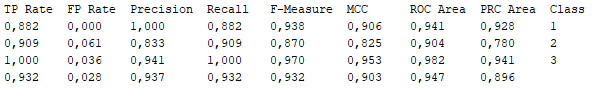
\includegraphics[width=\textwidth]{img/EC4.5.PNG}
    \caption{Estadísticas de clasificación de cada clase}
    
\end{figure}

Con ayuda de la matriz de confusión proporcionada por Weka vemos como de diecisiete instancias a clasificar de la clase a(1) quince han sido clasificadas bien frente a dos que han sido clasificadas de manera errónea en la clase b(2), con respecto a la clase b(2) vemos cómo de once instancias, diez han sido bien clasificadas frente a una que ha sido clasificada como de clase c(3), por último destacar que en la clase c(3) todas han sido bien clasificada haciendo un total de dieciséis.

A continuación se muestra la matriz de confusión para una mejor comprensión de lo anterior. 

\begin{figure}[H]
    \centering
    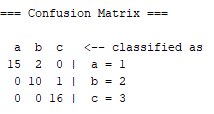
\includegraphics[width=\textwidth]{img/MC4.5.PNG}
    \caption{Estadísticas de clasificación de cada clase}
\end{figure}

\subsection{Ejercicio 2}

Escoja una de las bases de datos de clasificación para el trabajo de las dispuestas en Moodle. Se entiende que además de pasarla a formato .arff ya ha aplicado el preprocesamiento necesario en función del fichero "Pistas sobre los datasets con posible preprocesamiento a simple vista.pdf", en el caso que sea una de las bases de datos que lo requiera.
Cargue la base de datos con un 75/25\% y ejecute el algoritmo MultilayerPerceptron con los valores por defecto.
¿Qué observa al ir modificando solo el TrainingTime? ¿Cambia el valor de Correctly Classified instances al modificar el parámetro? ¿se estanca el aprendizaje o sobre entrena?
¿Qué observa al ir modificando solo el LeraningRate? ¿Cambia el valor de Correctly Classified instances al modificar el parámetro? ¿se estanca el aprendizaje o sobre entrena?

Para realizar este ejercicio hemos escogido la base de datos wine.arff utilizada con anteriores ejemplos.
De manera inicial con todos los valores por defecto y con un valor para TrainingTime de 500 tal y como viene por defecto el algoritmo nos clasifica 43 de las 44 destinadas a prueba de manera correcta, a medida que aumentamos el TrainingTime el valor del CCR sigue constante por lo que el algoritmo se estanca, por tanto hemos optado por reducirlo a la unidad e ir incrementando hasta comprobar donde este algoritmo de estanca que ha sido en un valor de siete. En la figura de abajo se muestra con más claridad la evolución del CCR.
\begin{figure}[H]
    \centering
    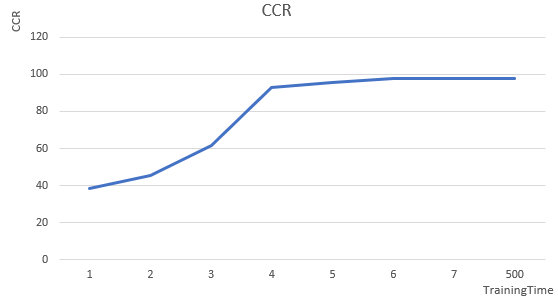
\includegraphics[width=\textwidth]{img/GM.PNG}
    \caption{Evolución del CCR con respecto a TrainingTime}

\end{figure}